\section{Borneo}

9 mai 2008

\begin{multicols}{2}

Bonjour tout le monde,

Aujourd'hui je vais vous parler de Bornéo, avec beaucoup de retard.

Après le précédent article qui parlait plus de la vie en mer, nous abordons aujourd'hui les côtes de Bornéo, connue anciennement pour ses pirates, maintenant pour sa grande réserve d'Orang Outans, il s'agit, avec Sumatra, d'un des deux seuls endroits au monde où il reste des Orang Outans en liberté.

Et nous, nous sommes là, nous sommes arrivés un peu à la rache, ne sachant pas trop où aborder (l'île est immense, regardez sur une carte) pour voir des singes. Nous arrivons à Kumai, et coup de chance c'est en bordure de la réserve nationale, nous pourrons donc y aller sans difficultés.

Pied à terre après nos 100 heures à bord. Nous découvrons un village tout en longueur le long de la mer.

\smallbreak
\hspace*{-0.65cm}
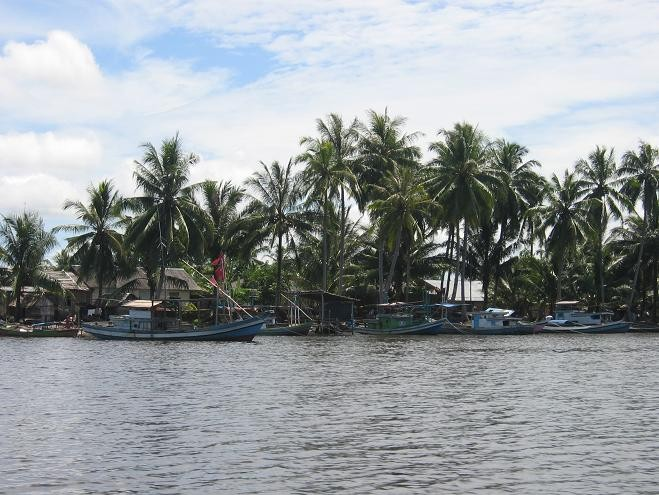
\includegraphics[width=5cm]{articles/Borneo/1210331303F4qq.jpg}
%La cote.
\smallbreak

\smallbreak
\hspace*{-0.65cm}
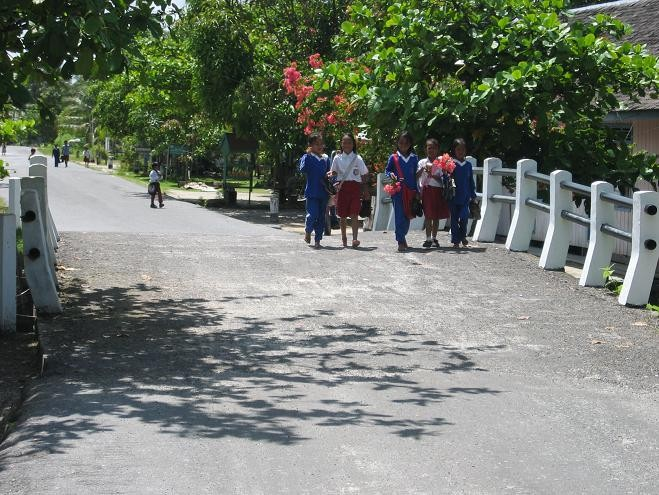
\includegraphics[width=5cm]{articles/Borneo/1210331297ISJ9.jpg}
%Rue centrale du village.
\smallbreak

Dès le lendemain nous nous sommes inscrits auprès d'un guide, pour pouvoir entrer dans la réserve et ainsi voir les Orang Outans. Ce qui paraissait au début être une belle arnaque s'est en fait avéré être une super journée, en pleine forêt tropicale.

\smallbreak
\hspace*{-0.65cm}
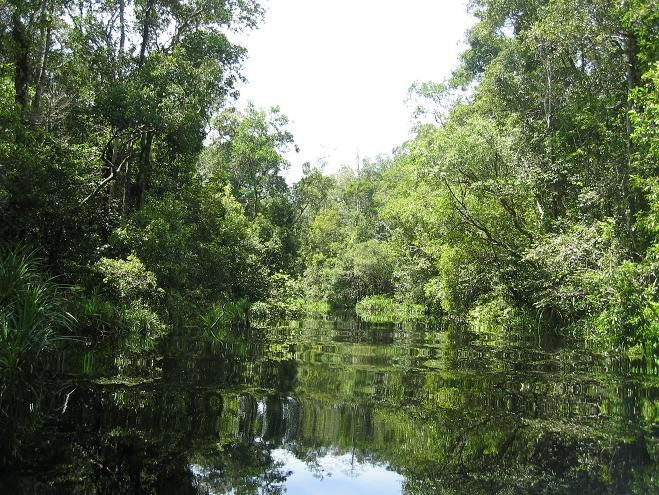
\includegraphics[width=5cm]{articles/Borneo/1210332087kPql.jpg}
%La mangrove.
\smallbreak

Nous avons assisté au repas de singes, en effet pendant la saison des fruits ils arrivent à se nourrir par eux même, mais en ce moment, la chose est plus difficile, les soigneurs apportent donc des bananes et les mettent sur des estrades, ce qui nous a permi, nous étions une poignée de personnes, de les regarder. En fait le plus impressionnant dans cette journée n'a pas été de les voir manger, mais plutôt de tomber au hasard d'un chemin sur l'un d'eux, de se faire un peu courser, puis de s'arrêter le regarder. Nous avons aussi vu des mamans garder leurs petits, c'était trop mignon.

\smallbreak
\hspace*{-0.65cm}
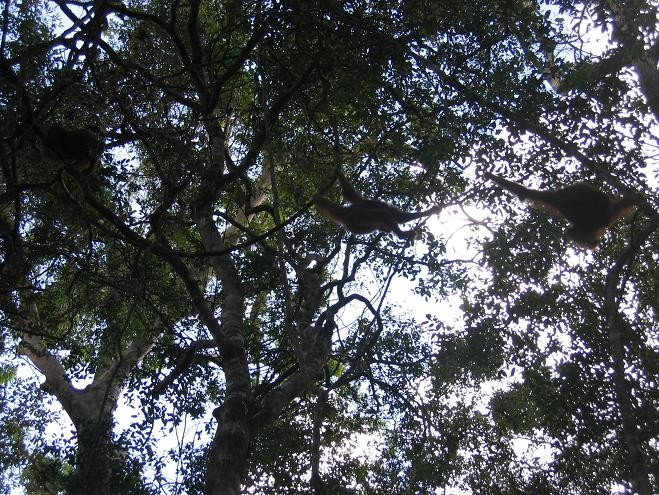
\includegraphics[width=5cm]{articles/Borneo/1210332096AngR.jpg}
%L'air de jeu des grands lascars.
\smallbreak

\smallbreak
\hspace*{-0.65cm}
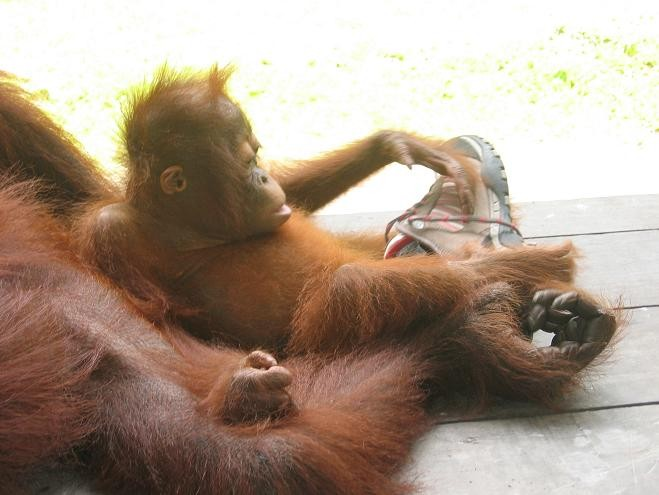
\includegraphics[width=5cm]{articles/Borneo/1210332100Imld.jpg}
%La nouvelle génération.
\smallbreak

%<div><object width="640" height="505"><param name="movie" value="http://www.dailymotion.com/swf/x5cnjc&v3=1&related=1"></param><param name="allowFullScreen" value="true"></param><param name="allowScriptAccess" value="always"></param><embed src="http://www.dailymotion.com/swf/x5cnjc&v3=1&related=1" type="application/x-shockwave-flash" width="640" height="505" allowFullScreen="true" allowScriptAccess="always"></embed></object></div>

\end{multicols}

\bigskip
\textbf{\textsc{Commentaires}}

\medskip
Nicoz a écrit le 19 juin 2008 :
\begin{displayquote}
Nan mais je rêve je suis le premier à poster sur cet article.
Bon je savais que t'avais bronzé et tout que t'avais pas forcément le temps de te raser sur le bateau mais là tout de même t'aurais pu me dire que tu t'étais teint en rousse :p
J'déconne mais ils sont trop mignons.
Bonne continuation
Continue à nous régaler des tes images.
\end{displayquote}

\vfill

